\chapter{Operations with Functions}

Given $f(x)=x^2 + 2x - 3$ and $g(x) = 5x+2$, simplify or evaluate each.

\begin{multicols}{4}
\begin{enumerate}
	\item $(f+g)(x)$
	\item $(f-g)(x) $
	\item $(g-f)(x)$
	\item $(fg)(x)$
\end{enumerate}	\setcounter{Review}{\value{enumi}}
\end{multicols}
\begin{multicols}{4}
\begin{enumerate}	\setcounter{enumi}{\value{Review}}
	\item $\left(\frac{f}{g}\right)(x)$
	\item $\left(\frac{g}{f}\right)(x) $
	\item $(g+f)(7)$
	\item $(fg)(0)$
\end{enumerate}	\setcounter{Review}{\value{enumi}}
\end{multicols}

Given $f(x) = x^2 + 5$ and $g(x) = -3x-2$, find or evaluate each.
\begin{multicols}{4}
\begin{enumerate}	\setcounter{enumi}{\value{Review}}
	\item $(f + g)(x)$
	\item $(fg)(x)$
	\item $(f-g)(4)$
	\item $\left(\frac{f}{g}\right)(7)$
\end{enumerate}	\setcounter{Review}{\value{enumi}}
\end{multicols}

Given the graph of $f(x)$ and $g(x)$, find each.
\begin{center}
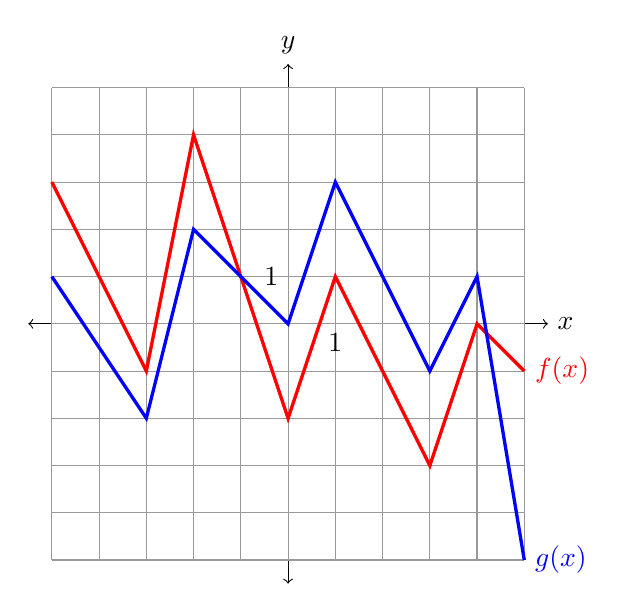
\begin{tikzpicture}[scale=0.6]
\draw[<->] (-5.5,0) -- (5.5,0) node [right] {$x$};
\draw[<->] (0,-5.5) -- (0,5.5) node [above] {$y$};
\draw[gray!80] (-5,-5) grid (5,5);
\node at (1,0) [below] {$1$};
\node at (0,1) [left] {$1$};
\coordinate (A) at (-5,3);
\coordinate (B) at (-3,-1);
\coordinate (C) at (-2,4);
\coordinate (D) at (0,-2);
\coordinate (E) at (1,1);
\coordinate (F) at (3,-3);
\coordinate (G) at (4,0);
\coordinate (H) at (5,-1);
\draw[red, very thick] (A) -- (B) -- (C) -- (D) -- (E) -- (F) -- (G) -- (H) node [right] {$f(x)$};
\coordinate (I) at (-5,1);
\coordinate (J) at (-3,-2);
\coordinate (K) at (-2,2);
\coordinate (L) at (0,0);
\coordinate (M) at (1,3);
\coordinate (N) at (3,-1);
\coordinate (O) at (4,1);
\coordinate (P) at (5,-5);
\draw[blue, very thick] (I) -- (J) -- (K) -- (L) -- (M) -- (N) -- (O) -- (P) node [right] {$g(x)$};
\end{tikzpicture}
\end{center}

\begin{multicols}{6}
\begin{enumerate}	\setcounter{enumi}{\value{Review}}
	\item $(f + g)(-2)$
	\item $(f - g)(1)$
	\item $(fg)(3)$
	\item $(g - f)(-5)$
	\item $\left(\frac{f}{g}\right)(4)$
	\item $\left(\frac{g}{f}\right)(-5)$
\end{enumerate}	\setcounter{Review}{\value{enumi}}
\end{multicols}

Find the value of each of the following given the table below.
\begin{center}
\begin{tabular}{c|c|c|c|c|c|c|c|c|c}
    $\mathbf{x}$ & $\mathbf{-4}$ & $\mathbf{-3}$ & $\mathbf{-2}$ & $\mathbf{-1}$ & \textbf{0} & \textbf{1} & \textbf{2} & \textbf{3} & \textbf{4} \\ \hline
    $\mathbf{f(x)}$ & $-1$ & 3 & 1 & 4 & $-2$ & $-4$ & $-3$ & 2 & 0 \\ \hline
    $\mathbf{g(x)}$ & 0 & $-4$ & 1 & $-3$ & $-2$ & 4 & 2 & $-1$ & 3 \\
\end{tabular}
\end{center}

\begin{multicols}{5}
\begin{enumerate}	\setcounter{enumi}{\value{Review}}
	\item $(f + g)(1)$
	\item $(f - g)(-2)$
	\item $(fg)(0)$
	\item $\left(\frac{g}{f}\right)(2)$
	\item $(g + g)(-3)$
\end{enumerate}		\setcounter{Review}{\value{enumi}}
\end{multicols}

\newpage

\section{Answer Key}

\begin{enumerate}
	\item $x^2+7x-1$
    \item $x^2-3x-5$
    \item $-x^2+3x+5$
    \item $5x^3+12x^2-11x-6$
    \item $\frac{x^2+2x+3}{5x+2}$
    \item $\frac{5x+2}{x^2+2x+3}$
    \item 97
    \item $-6$
    \item $x^2-3x+3$
    \item $-3x^3-2x^2-15x-10$
    \item 35
    \item $-\frac{54}{23}$
    \item 6
    \item $-2$
    \item 3
    \item $-2$
    \item 0
    \item $\frac{1}{3}$
    \item 0
    \item 0
    \item 4
    \item $-\frac{2}{3}$
    \item $-8$
\end{enumerate}